\documentclass[11pt,a4paper]{article}
\usepackage{fontspec,polyglossia}
\setdefaultlanguage{russian}
\setotherlanguage{english}
\defaultfontfeatures{Ligatures=TeX}
\setmainfont[Path=fonts/,UprightFont=cmunrm.otf,BoldFont=cmunbx.otf,ItalicFont=cmunti.otf,BoldItalicFont=cmunbi.otf]{CMU Serif}
\usepackage[left=2cm,right=2cm,top=2cm,bottom=3cm]{geometry}
\usepackage{amsmath,amssymb,booktabs,array,graphicx,float,caption,setspace,tikz}
\usetikzlibrary{arrows.meta,positioning}
\usepackage[unicode,hidelinks]{hyperref}
\setlength{\parindent}{0pt}
\setlength{\parskip}{0.2\baselineskip}
\setlength{\emergencystretch}{3em}
\renewcommand{\arraystretch}{1.12}
\captionsetup{font=small}
\newcommand{\sI}{\text{(1)}}
\newcommand{\sII}{\text{(2)}}
\newcommand{\secs}{\text{с}}
\begin{document}
\hypersetup{pageanchor=false}
\begin{titlepage}
\centering
Федеральное государственное автономное\\
образовательное учреждение высшего образования\\
\textbf{«Национальный исследовательский университет ИТМО»}
\vfill
{\Large\bfseries Отчёт по учебно-исследовательской работе № 2\par}
\vspace{0.7\baselineskip}
по дисциплине «Моделирование»\\[0.7\baselineskip]
{\large\bfseries «Марковские модели систем\\массового обслуживания»\par}
\vspace{0.7\baselineskip}
Вариант 40/79/16
\vfill
\begin{flushright}
Выполнил:\\
Чэнь Хаолинь P3316\\[1\baselineskip]
Проверил:\\
Тропченко Андрей Александрович
\end{flushright}
\vfill
г. Санкт-Петербург, 2026
\end{titlepage}
\hypersetup{pageanchor=true}
\setstretch{0.95}
\tableofcontents
\newpage
\setstretch{1}

\section{Постановка задачи и исходные данные}
Цель работы --- изучить метод марковских случайных процессов и применить его к исследованию систем массового обслуживания с однородным потоком заявок.

Необходимо разработать марковские модели двух систем: описать состояния, построить размеченные графы переходов и матрицы интенсивностей, определить стационарные вероятности и характеристики обслуживания. На основании расчётов и графиков следует сравнить системы и выбрать организацию, обеспечивающую \textbf{минимальную суммарную среднюю длину очередей}.

В обе системы поступает простейший поток с интенсивностью $\lambda=0{,}1\ \secs^{-1}$. Средняя длительность обслуживания каждой заявки равна $b=40\ \secs$. Для экспоненциального обслуживания $\mu=1/b=0{,}025\ \secs^{-1}$. Вероятности направления к двум приборам обозначим $a_1=0{,}7$ и $a_2=0{,}3$.

\begin{table}[H]\centering
\caption{Структура и параметры исследуемых систем}
\small
\begin{tabular}{>{\raggedright\arraybackslash}p{4.4cm}>{\raggedright\arraybackslash}p{5.4cm}>{\raggedright\arraybackslash}p{5.4cm}}
\toprule
Параметр & СИСТЕМА 1 & СИСТЕМА 2\\\midrule
Число приборов & 2 & 2\\
Накопитель & Общий, ёмкость $r=4$ & Раздельные, $r_1=0$, $r_2=2$\\
Обслуживание П1 & Экспоненциальное & Гиперэкспоненциальное, $v=2{,}6$\\
Обслуживание П2 & Экспоненциальное & Экспоненциальное\\
Порядок обслуживания & FIFO в общей очереди & FIFO перед П2\\
Отказ & Оба прибора заняты, очередь полна & Выбранный прибор и его накопитель заполнены\\
\bottomrule
\end{tabular}
\end{table}

В СИСТЕМЕ 1 заявка занимает свободный прибор. Если свободны оба прибора, выбор производится с вероятностями $a_1$ и $a_2$. Если оба заняты, заявка помещается в общий накопитель. Освободившийся прибор немедленно принимает первую заявку из общей очереди.

В СИСТЕМЕ 2 поток независимо разделяется: $\lambda_1=a_1\lambda=0{,}07\ \secs^{-1}$ и $\lambda_2=a_2\lambda=0{,}03\ \secs^{-1}$. Перенаправление между приборами отсутствует. Гиперэкспоненциальный закон реализуется в П1. Длительности обслуживания и входной поток независимы.

\subsection{Обозначения и уравнения стационарного режима}
Используются состояния $E_i$, вероятности $p_i$ и матрица интенсивностей $G=\{g_{ij}\}$, где $g_{ij}$ при $i\ne j$ задаёт интенсивность перехода из $E_i$ в $E_j$. Диагональные элементы и стационарные вероятности удовлетворяют условиям
\begin{equation}
g_{ii}=-\sum_{j\ne i}g_{ij},\qquad
\sum_i p_i g_{ij}=0,\qquad \sum_i p_i=1.
\label{eq:balance}
\end{equation}
Отказы не меняют состояние и не включаются в сумму интенсивностей выхода. Для характеристик используются обозначения $y$ (нагрузка), $\rho$ (загрузка), $\eta$ (простой), $l$ (средняя длина очереди), $m$ (среднее число заявок), $\pi$ (вероятность потери), $\lambda'$ (производительность), $\lambda''$ (поток отказов), $w$ (время ожидания), $u$ (время пребывания).

\newpage
\section{Марковская модель СИСТЕМЫ 1}
\subsection{Состояния и размеченный граф}
Код состояния $(d_1,d_2;q)$ содержит признаки занятости приборов $d_1,d_2\in\{0,1\}$ и число заявок в общем накопителе $q$. Получаются восемь состояний:
\[
E_0=(0,0;0),\quad E_1=(1,0;0),\quad E_2=(0,1;0),\quad
E_{q+3}=(1,1;q),\quad q=0,\ldots,4.
\]
Разделение состояний $E_1$ и $E_2$ позволяет вычислять загрузку каждого прибора. При $q>0$ оба прибора обязательно заняты.

\begin{figure}[H]\centering
\begin{tikzpicture}[>=Stealth,st/.style={circle,draw,minimum size=9mm,font=\small},every edge/.style={draw,->},every node/.style={font=\small}]
\node[st](e0) at (0,0){$E_0$};
\node[st](e1) at (2,1.25){$E_1$};
\node[st](e2) at (2,-1.25){$E_2$};
\node[st](e3) at (4,0){$E_3$};
\node[st](e4) at (6,0){$E_4$};
\node[st](e5) at (8,0){$E_5$};
\node[st](e6) at (10,0){$E_6$};
\node[st](e7) at (12,0){$E_7$};
\path (e0) edge[bend left=14] node[above left]{$a_1\lambda$}(e1)
 (e1) edge[bend left=14] node[below right]{$\mu$}(e0)
 (e0) edge[bend right=14] node[below left]{$a_2\lambda$}(e2)
 (e2) edge[bend right=14] node[above right]{$\mu$}(e0)
 (e1) edge[bend left=14] node[above right]{$\lambda$}(e3)
 (e3) edge[bend left=14] node[below left]{$\mu$}(e1)
 (e2) edge[bend right=14] node[below right]{$\lambda$}(e3)
 (e3) edge[bend right=14] node[above left]{$\mu$}(e2);
\foreach \x/\y in {3/4,4/5,5/6,6/7}{
\path (e\x) edge[bend left=18] node[above]{$\lambda$}(e\y)
(e\y) edge[bend left=18] node[below]{$2\mu$}(e\x);}
\end{tikzpicture}
\caption{Размеченный граф СИСТЕМЫ 1. В состоянии $E_7$ поступающая заявка теряется}
\end{figure}

\subsection{Матрица интенсивностей переходов}
Порядок строк и столбцов: $E_0,E_1,\ldots,E_7$. Все элементы матрицы имеют размерность $\secs^{-1}$:
\begin{equation}
G^{\sI}=\begin{pmatrix}
-0.1&0.07&0.03&0&0&0&0&0\\
0.025&-0.125&0&0.1&0&0&0&0\\
0.025&0&-0.125&0.1&0&0&0&0\\
0&0.025&0.025&-0.15&0.1&0&0&0\\
0&0&0&0.05&-0.15&0.1&0&0\\
0&0&0&0&0.05&-0.15&0.1&0\\
0&0&0&0&0&0.05&-0.15&0.1\\
0&0&0&0&0&0&0.05&-0.05
\end{pmatrix}.
\end{equation}
Например, переход $E_3\to E_1$ означает завершение обслуживания в П2, а $E_4\to E_3$ --- завершение обслуживания в любом приборе с немедленным занятием освободившегося прибора заявкой из очереди.

При объединении $E_1$ и $E_2$ по общему числу заявок получается процесс рождения и гибели: интенсивности поступления равны $\lambda$, а завершения обслуживания --- $\mu$ при одной заявке и $2\mu$ при двух и более. Независимая проверка даёт
\[
p_0=\frac1{253},\quad p_1+p_2=\frac4{253},\quad
(p_3,p_4,p_5,p_6,p_7)=\frac1{253}(8,16,32,64,128).
\]

\newpage
\section{Марковская модель СИСТЕМЫ 2}
\subsection{Гиперэкспоненциальное обслуживание}
Одна заявка в П1 выбирает одну из двух экспоненциальных ветвей; это альтернативные режимы одного прибора, а не два параллельных прибора. Для длительности обслуживания $T$ принимается
\begin{equation}
F_T(t)=1-h_1e^{-\mu_{11}t}-h_2e^{-\mu_{12}t},\qquad t\ge0,\qquad h_1+h_2=1.
\end{equation}
Среднее $b$ и коэффициент вариации $v$ фиксируют первые два момента, но не задают единственную двухветвевую смесь. Используется параметризация с равными вкладами ветвей в среднее: $h_1/\mu_{11}=h_2/\mu_{12}=b/2$. Тогда
\begin{align}
h_1&=\frac12\left(1+\sqrt{\frac{v^2-1}{v^2+1}}\right)=0{,}9307748952,
&h_2&=0{,}0692251048,\\
\mu_{11}&=\frac{2h_1}{b}=0{,}04653874476\ \secs^{-1},
&\mu_{12}&=\frac{2h_2}{b}=0{,}00346125524\ \secs^{-1}.
\end{align}
Проверка моментов:
\[
\mathsf E[T]=\frac{h_1}{\mu_{11}}+\frac{h_2}{\mu_{12}}=40\ \secs,\qquad
\mathsf E[T^2]=2\left(\frac{h_1}{\mu_{11}^2}+\frac{h_2}{\mu_{12}^2}\right)=12416\ \secs^2,
\]
\[
\mathsf D[T]=12416-1600=10816\ \secs^2,\qquad
\frac{\sqrt{\mathsf D[T]}}{\mathsf E[T]}=\frac{104}{40}=2{,}6.
\]

\subsection{Состояния и размеченный граф}
Состояние кодируется парой $(a,k)$: $a=0$ означает свободный П1, $a=1,2$ --- обслуживание по соответствующей ветви; $k=0,1,2,3$ --- число заявок у П2, включая обслуживаемую. Нумерация $E_{4a+k}=(a,k)$ даёт 12 состояний. Добавление ветви к коду сохраняет марковское свойство.

\begin{figure}[H]\centering
\begin{tikzpicture}[>=Stealth,st/.style={draw,rounded corners=2pt,minimum width=16mm,minimum height=8mm,font=\small},every edge/.style={draw,->},every node/.style={font=\small}]
\foreach \k in {0,1,2,3}{
\pgfmathtruncatemacro{\n}{\k+4}
\pgfmathtruncatemacro{\m}{\k+8}
\node[st](t\k) at (3.4*\k,2.0){$E_{\n}$};
\node[st](c\k) at (3.4*\k,0){$E_{\k}$};
\node[st](b\k) at (3.4*\k,-2.0){$E_{\m}$};
\path (c\k) edge[bend left=13] node[left]{$\lambda_1h_1$}(t\k)
 (t\k) edge[bend left=13] node[right]{$\mu_{11}$}(c\k)
 (c\k) edge[bend right=13] node[left]{$\lambda_1h_2$}(b\k)
 (b\k) edge[bend right=13] node[right]{$\mu_{12}$}(c\k);
}
\foreach \row in {t,c,b}{\foreach \x/\y in {0/1,1/2,2/3}{
\path (\row\x) edge[bend left=12] node[above]{$\lambda_2$}(\row\y)
 (\row\y) edge[bend left=12] node[below]{$\mu$}(\row\x);}}
\end{tikzpicture}
\caption{Граф СИСТЕМЫ 2. Верхний ряд: $a=1$, средний: $a=0$, нижний: $a=2$}
\end{figure}
Поступление к занятому П1 всегда вызывает отказ; поступление к П2 вызывает отказ при $k=3$. Оба типа отказов оставляют состояние неизменным.

\newpage
\subsection{Матрица интенсивностей переходов}
В порядке $E_0,\ldots,E_{11}$ матрица записывается блоками $4\times4$:
\begin{equation}
G^{\sII}=\begin{pmatrix}
C-\lambda_1I_4&\lambda_1h_1I_4&\lambda_1h_2I_4\\
\mu_{11}I_4&C-\mu_{11}I_4&0\\
\mu_{12}I_4&0&C-\mu_{12}I_4
\end{pmatrix},\quad
C=\begin{pmatrix}
-0.03&0.03&0&0\\
0.025&-0.055&0.03&0\\
0&0.025&-0.055&0.03\\
0&0&0.025&-0.025
\end{pmatrix}.
\end{equation}
Здесь $I_4$ --- единичная матрица, $0$ --- нулевой блок. Численные значения оставшихся коэффициентов:
\[
\lambda_1=0{,}07,\quad \lambda_1h_1=0{,}06515424266,\quad
\lambda_1h_2=0{,}00484575734;
\]
\[
\mu_{11}=0{,}04653874476,\qquad \mu_{12}=0{,}00346125524.
\]
Все интенсивности выражены в $\secs^{-1}$. Блочная запись полностью определяет каждый элемент матрицы $12\times12$.

\section{Стационарные вероятности состояний}
Для каждой системы решена система уравнений~\eqref{eq:balance}. В обеих моделях все состояния сообщаются, поэтому стационарное распределение единственно.

\begin{table}[H]\centering
\caption{Форма 1. Стационарные вероятности состояний}
\small
\begin{tabular}{ccrccr}
\toprule
\multicolumn{3}{c}{СИСТЕМА 1}&\multicolumn{3}{c}{СИСТЕМА 2}\\
Состояние&Код $(d_1,d_2;q)$&$p_i^{\sI}$&Состояние&Код $(a,k)$&$p_i^{\sII}$\\\midrule
$E_{0}$ & $(0,0;0)$ & 0.003952569 & $E_{0}$ & $(0,0)$ & 0.049023453 \\
$E_{1}$ & $(1,0;0)$ & 0.008537549 & $E_{1}$ & $(0,1)$ & 0.058828143 \\
$E_{2}$ & $(0,1;0)$ & 0.007272727 & $E_{2}$ & $(0,2)$ & 0.070593772 \\
$E_{3}$ & $(1,1;0)$ & 0.031620553 & $E_{3}$ & $(0,3)$ & 0.084712526 \\
$E_{4}$ & $(1,1;1)$ & 0.063241107 & $E_{4}$ & $(1,0)$ & 0.068632834 \\
$E_{5}$ & $(1,1;2)$ & 0.126482213 & $E_{5}$ & $(1,1)$ & 0.082359401 \\
$E_{6}$ & $(1,1;3)$ & 0.252964427 & $E_{6}$ & $(1,2)$ & 0.098831281 \\
$E_{7}$ & $(1,1;4)$ & 0.505928854 & $E_{7}$ & $(1,3)$ & 0.118597537 \\
--- & --- & --- & $E_{8}$ & $(2,0)$ & 0.068632834 \\
--- & --- & --- & $E_{9}$ & $(2,1)$ & 0.082359401 \\
--- & --- & --- & $E_{10}$ & $(2,2)$ & 0.098831281 \\
--- & --- & --- & $E_{11}$ & $(2,3)$ & 0.118597537 \\
\bottomrule

\end{tabular}
\end{table}

В СИСТЕМЕ 2 маргинальные вероятности обозначим
\[
A_a=\sum_{k=0}^{3}p_{4a+k}^{\sII},\qquad B_k=\sum_{a=0}^{2}p_{4a+k}^{\sII}.
\]
Их значения:
\[
(A_0,A_1,A_2)=(0{,}263157895;\ 0{,}368421053;\ 0{,}368421053),
\]
\[
(B_0,B_1,B_2,B_3)=(0{,}186289121;\ 0{,}223546945;\ 0{,}268256334;\ 0{,}321907601).
\]
Проверено: $p_{4a+k}^{\sII}=A_aB_k$, $\sum_i p_i=1$. Для обеих моделей невязка стационарных уравнений до округления меньше $10^{-16}\ \secs^{-1}$.

\newpage
\section{Расчёт характеристик через вероятности состояний}
\subsection{СИСТЕМА 1}
В этом подразделе $p_i=p_i^{\sI}$. Нагрузка всей системы $y=\lambda b=4$. Загрузка каждого прибора, среднее число работающих приборов $k'$ и средняя загрузка системы равны
\begin{align}
\rho_1&=p_1+\sum_{i=3}^{7}p_i,&
\rho_2&=p_2+\sum_{i=3}^{7}p_i,\\
k'&=\rho_1+\rho_2,& \rho&=\frac{\rho_1+\rho_2}{2},\qquad \eta=1-\rho.
\end{align}
Величина $\eta$ --- средняя доля простаивающих приборов. Вероятность одновременного простоя обоих приборов равна $p_0$ и отличается от $\eta$.

Числа ожидающих и находящихся в системе заявок рассчитываются непосредственным суммированием по состояниям:
\begin{equation}
l=\sum_{q=0}^{4}q p_{q+3},\qquad
m=p_1+p_2+\sum_{q=0}^{4}(q+2)p_{q+3}.
\end{equation}
По вероятности состояния, в котором происходит отказ, и интенсивностям завершения обслуживания получаем
\begin{equation}
\pi=p_7,\qquad \lambda_i'=\mu\rho_i,\qquad
\lambda'=\mu(\rho_1+\rho_2),\qquad \lambda''=\lambda p_7.
\end{equation}

Для времени ожидания рассмотрим поступающую принятую заявку. При наличии свободного прибора она начинает обслуживание немедленно. Если оба прибора заняты и в очереди $q\le3$ заявок, ей необходимо дождаться $q+1$ завершений обслуживания. До начала её обслуживания оба прибора заняты, а средний интервал между завершениями равен $1/(2\mu)$. Поэтому
\begin{equation}
w=\frac{\displaystyle\sum_{q=0}^{3}p_{q+3}\frac{q+1}{2\mu}}{1-p_7}
=62{,}72\ \secs,\qquad u=w+b=102{,}72\ \secs.
\label{eq:wait1}
\end{equation}
Деление на $1-p_7$ учитывает условие принятия заявки. Формула~\eqref{eq:wait1} выведена по состоянию, наблюдаемому поступающей заявкой, без использования формулы Литтла.

Для сравнения времени обслуживания в отдельных приборах обозначим
\[
S=\sum_{q=0}^{3}p_{q+3}\frac{q+1}{2\mu}.
\]
Если заявка ожидает, вероятность её последующего обслуживания каждым прибором равна $1/2$, поскольку интенсивности обслуживания одинаковы. Средние времена среди заявок, в итоге обслуженных П$i$, равны
\begin{equation}
w_i=\frac{\lambda S}{2\lambda_i'},\qquad u_i=w_i+b.
\end{equation}
Для учёта ожидающих заявок по будущему обслуживающему прибору можно ввести $l_i^*=l/2$ и $m_i^*=\rho_i+l_i^*$. Это условное распределение общей очереди, а не физические отдельные накопители. Отдельные входные нагрузки и вероятности отказа по будущему прибору для общей очереди не определяются: отказавшая заявка до прибора не доходит.

\newpage
\subsection{СИСТЕМА 2}
Используем маргинальные вероятности $A_a$ и $B_k$, полученные суммированием стационарных вероятностей полной модели. Нагрузки, загрузки и среднее число работающих приборов:
\begin{align}
y_1&=\lambda_1b=2{,}8,&y_2&=\lambda_2b=1{,}2,&y&=y_1+y_2=4,\\
\rho_1&=A_1+A_2,&\rho_2&=B_1+B_2+B_3,&k'&=\rho_1+\rho_2,\\
\rho&=\frac{\rho_1+\rho_2}{2},&&&\eta&=1-\rho.
\end{align}
Средние длины очередей и числа заявок:
\begin{equation}
l_1=0,\quad l_2=B_2+2B_3,\quad l=l_2,\qquad
m_1=A_1+A_2,\quad m_2=B_1+2B_2+3B_3,\quad m=m_1+m_2.
\end{equation}
Пуассоновская заявка наблюдает состояния с их стационарными вероятностями. Условные вероятности отказа для выбранного прибора и вероятность отказа для всего входного потока имеют вид
\begin{equation}
\pi_1=A_1+A_2,\qquad \pi_2=B_3,\qquad
\pi=a_1\pi_1+a_2\pi_2.
\end{equation}
Вероятности $\pi_1$ и $\pi_2$ нельзя просто складывать: они относятся к разным частям потока. Производительности вычисляются непосредственно по интенсивностям завершения обслуживания в состояниях:
\begin{equation}
\lambda_1'=\mu_{11}A_1+\mu_{12}A_2,\qquad
\lambda_2'=\mu(B_1+B_2+B_3),\qquad
\lambda'=\lambda_1'+\lambda_2'.
\end{equation}
Интенсивности отказов равны $\lambda_i''=\lambda_i\pi_i$, $\lambda''=\lambda_1''+\lambda_2''$.

У П1 нет накопителя, поэтому принятые заявки не ожидают: $w_1=0$, $u_1=b$. У П2 принятая заявка, увидевшая $k=0,1,2$, ожидает завершения $k$ обслуживаний. За счёт отсутствия последействия у экспоненциального распределения среднее остаточное время текущего обслуживания также равно $b$. Следовательно,
\begin{equation}
w_2=\frac{b(B_1+2B_2)}{B_0+B_1+B_2}=44{,}835165\ \secs,\qquad
u_2=w_2+b=84{,}835165\ \secs.
\end{equation}
Средние времена по системе определяются среди \emph{принятых} заявок. Их доли по приборам пропорциональны производительностям, а не исходным вероятностям $a_i$:
\begin{equation}
w=\frac{\lambda_1'w_1+\lambda_2'w_2}{\lambda'}=23{,}528936\ \secs,\qquad
u=\frac{\lambda_1'u_1+\lambda_2'u_2}{\lambda'}=63{,}528936\ \secs.
\end{equation}

Для узла П1 без очереди баланс даёт
\[
A_1=\frac{\lambda_1h_1}{\mu_{11}}A_0,\quad
A_2=\frac{\lambda_1h_2}{\mu_{12}}A_0,\quad
A_0=\frac{1}{1+\lambda_1b}.
\]
Поэтому при фиксированном $b$ его вероятность отказа и производительность не зависят от коэффициента вариации. Величина $v$ определяет параметры и фазовые состояния модели, но при выбранном размещении гиперэкспоненциального прибора не меняет итоговые средние характеристики системы.

\newpage
\section{Численные результаты и проверка}
\subsection{Характеристики систем}
\begin{table}[H]\centering
\caption{Форма 2. Суммарные и средние характеристики систем}
\small\setlength{\tabcolsep}{4pt}
\begin{tabular}{>{\raggedright\arraybackslash}p{4.8cm}crr}
\toprule
Характеристика & Обозначение & СИСТЕМА 1 & СИСТЕМА 2\\\midrule
Нагрузка & $y$ & 4.000000000 & 4.000000000 \\
Средняя загрузка приборов & $\rho$ & 0.988142292 & 0.775276492 \\
Среднее число работающих приборов & $k'$ & 1.976284585 & 1.550552985 \\
Коэффициент простоя & $\eta$ & 0.011857708 & 0.224723508 \\
Средняя длина очереди & $l$ & 3.098814229 & 0.912071535 \\
Среднее число заявок & $m$ & 5.075098814 & 2.462624520 \\
Вероятность потери & $\pi$ & 0.505928854 & 0.612361754 \\
Производительность, с$^{-1}$ & $\lambda'$ & 0.049407115 & 0.038763825 \\
Поток отказов, с$^{-1}$ & $\lambda''$ & 0.050592885 & 0.061236175 \\
Среднее время ожидания, с & $w$ & 62.720000000 & 23.528935654 \\
Среднее время пребывания, с & $u$ & 102.720000000 & 63.528935654 \\
\bottomrule

\end{tabular}
\end{table}
Загрузка $\rho$ приведена как средняя по двум приборам, а её сумма вынесена отдельно в строку $k'$. Времена $w,u$ усреднены по принятым заявкам; отказавшие заявки в эти средние не включены. Формулы вычисления всех строк приведены в разделе 5.

\subsection{Контрольные соотношения}
Фундаментальные зависимости используются только для проверки результатов, полученных через вероятности состояний. Баланс потоков выполняется:
\begin{align*}
\text{СИСТЕМА 1:}\quad&0{,}049407115+0{,}050592885=0{,}1,\\
\text{СИСТЕМА 2:}\quad&0{,}038763825+0{,}061236175=0{,}1.
\end{align*}
Дополнительно проверены $\lambda'=\lambda(1-\pi)$, $m=l+k'$ и формулы Литтла:
\begin{align*}
\text{СИСТЕМА 1:}\quad
\lambda'w&=0{,}0494071146\cdot62{,}72=3{,}098814229=l,\\
\lambda'u&=0{,}0494071146\cdot102{,}72=5{,}075098814=m;\\[2pt]
\text{СИСТЕМА 2:}\quad
\lambda'w&=0{,}0387638246\cdot23{,}528935654=0{,}912071535=l,\\
\lambda'u&=0{,}0387638246\cdot63{,}528935654=2{,}462624520=m.
\end{align*}
Расхождения до округления не превышают $10^{-11}$ для приведённых проверок. Несмотря на нагрузку $y=4$, превышающую число приборов, стационарный режим существует: ёмкости накопителей конечны, избыток входного потока преобразуется в поток отказов.

\newpage
\subsection{Характеристики отдельных приборов}
\begin{table}[H]\centering
\caption{Форма 2 (продолжение). Показатели приборов}
\small\setlength{\tabcolsep}{5pt}
\begin{tabular}{llrrrr}
\toprule
& & \multicolumn{2}{c}{СИСТЕМА 1}&\multicolumn{2}{c}{СИСТЕМА 2}\\
Характеристика & Формула & П1 & П2 & П1 & П2\\\midrule
Нагрузка & $y_i=\lambda_i b$ & --- & --- & 2.800000 & 1.200000 \\
Загрузка & $\rho_i=\sum p$ & 0.988775 & 0.987510 & 0.736842 & 0.813711 \\
Простой & $\eta_i=1-\rho_i$ & 0.011225 & 0.012490 & 0.263158 & 0.186289 \\
Длина очереди & $l_i\ (l_i^*)$ & 1.549407 & 1.549407 & 0.000000 & 0.912072 \\
Число заявок & $m_i\ (m_i^*)$ & 2.538182 & 2.536917 & 0.736842 & 1.725782 \\
Ожидание, с & $w_i$ & 62.679885 & 62.760167 & 0.000000 & 44.835165 \\
Пребывание, с & $u_i=w_i+b$ & 102.679885 & 102.760167 & 40.000000 & 84.835165 \\
Вероятность потери & $\pi_i$ & --- & --- & 0.736842 & 0.321908 \\
Производит., с$^{-1}$ & $\lambda_i'$ & 0.024719 & 0.024688 & 0.018421 & 0.020343 \\
Поток отказов, с$^{-1}$ & $\lambda_i''=\lambda_i\pi_i$ & --- & --- & 0.051579 & 0.009657 \\
\bottomrule

\end{tabular}
\end{table}
Прочерк означает отсутствие однозначного разбиения общего входного потока по будущим обслуживающим приборам. В СИСТЕМЕ 1 $l_i$ и $m_i$ в таблице понимаются как $l_i^*$ и $m_i^*$: ожидающие заявки условно отнесены к прибору, который впоследствии их обслужит. Физическая общая очередь имеет длину $l=3{,}098814$, её нельзя считать двумя независимыми очередями.

Для СИСТЕМЫ 1 формула загрузки в строке таблицы раскрывается как $p_i+\sum_{j=3}^{7}p_j$ при $i=1,2$. Для СИСТЕМЫ 2 --- как $A_1+A_2$ и $B_1+B_2+B_3$. Формулы производительности различаются: $\mu\rho_i$ в первой системе и $\mu_{11}A_1+\mu_{12}A_2$, $\mu\rho_2$ во второй. Знак $\sum p$ в таблице означает суммирование по состояниям занятости соответствующего прибора.

Отдельные показатели показывают причину различий. Общая очередь почти полностью загружает оба прибора СИСТЕМЫ 1: загрузка каждого составляет около $0{,}99$. В СИСТЕМЕ 2 наиболее интенсивный поток $\lambda_1=0{,}07\ \secs^{-1}$ направляется к прибору без накопителя, поэтому около $73{,}68\%$ этого потока теряется. При этом П2 не может принять заявки, направленные к П1, даже если у П2 есть свободное место.

\section{Сравнительный анализ}
При заданных параметрах разность средних длин очередей равна
\[
l^{\sI}-l^{\sII}=3{,}098814229-0{,}912071535=2{,}186742694.
\]
Относительное уменьшение при переходе к СИСТЕМЕ 2 составляет
\[
\frac{l^{\sI}-l^{\sII}}{l^{\sI}}\cdot100\%=70{,}57\%.
\]
Среднее время пребывания принятых заявок уменьшается с $102{,}72$ до $63{,}53\ \secs$. Однако производительность снижается с $0{,}049407$ до $0{,}038764\ \secs^{-1}$, а вероятность потери увеличивается на $0{,}106433$, то есть примерно на $10{,}64$ процентного пункта. Меньшая очередь во второй системе связана как с меньшей ёмкостью накопителей, так и с более ранним отказом заявкам.

\newpage
\subsection{Зависимость характеристик от интенсивности поступления}
Для исследования чувствительности интенсивность $\lambda$ изменялась от $0{,}005$ до $0{,}2\ \secs^{-1}$ при неизменных $b$, вероятностях направления, законах обслуживания и ёмкостях накопителей. Для каждой точки повторно решалась система стационарных уравнений.

\begin{figure}[H]\centering
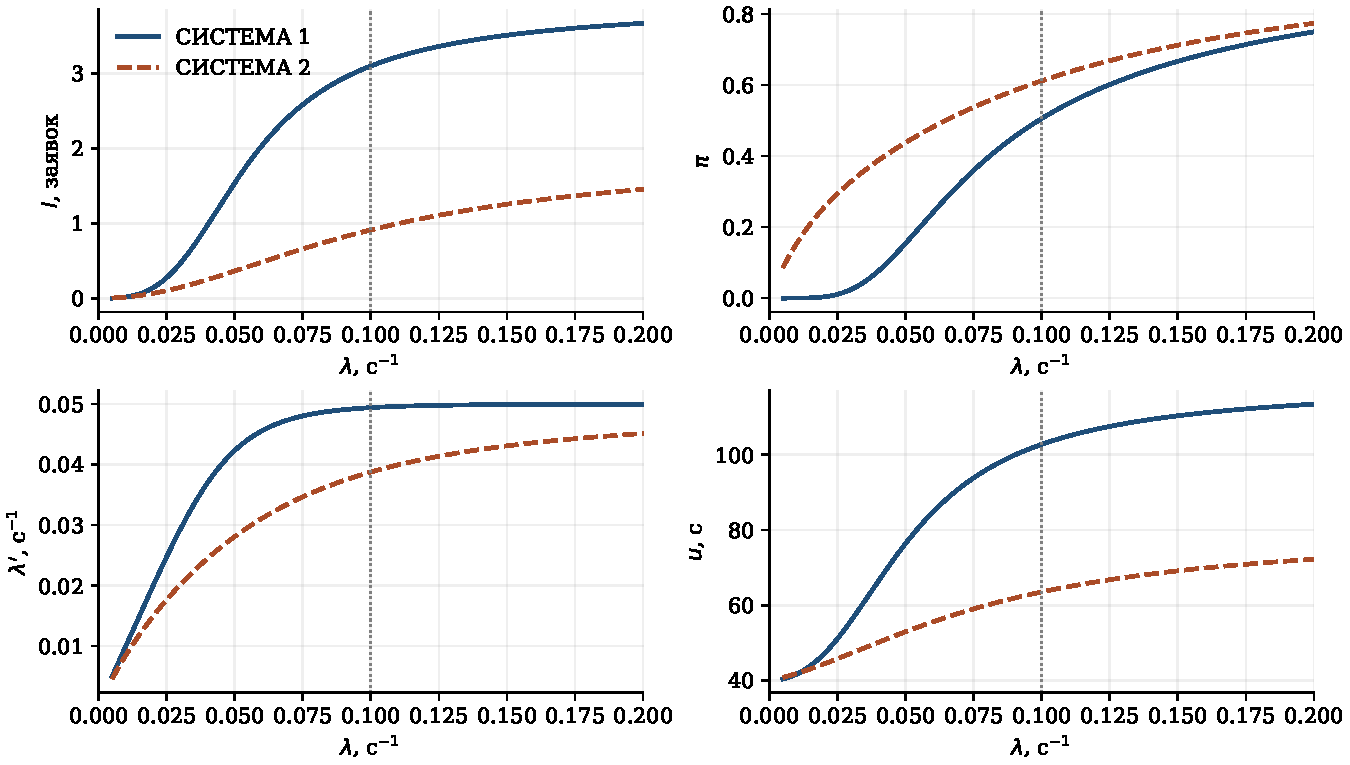
\includegraphics[width=\linewidth]{figures/comparison.pdf}
\caption{Зависимости длины очереди, потерь, производительности и времени пребывания от $\lambda$. Вертикальная пунктирная линия соответствует $\lambda=0{,}1\ \secs^{-1}$}
\end{figure}

\begin{table}[H]\centering
\caption{Контрольные точки зависимости $l(\lambda)$}
\small
\begin{tabular}{rrrrrrr}
\toprule
$\lambda$, $\secs^{-1}$&0.010&0.025&0.050&0.100&0.150&0.200\\\midrule
$l^{\sI}$&0.016555&0.273684&1.538462&3.098814&3.509382&3.668529\\
$l^{\sII}$&0.015717&0.101623&0.363971&0.912072&1.255391&1.453533\\
\bottomrule
\end{tabular}
\end{table}

При росте потока очереди и потери увеличиваются, $\lambda'\to2/b=0{,}05\ \secs^{-1}$, $l^{\sI}\to4$, $l^{\sII}\to2$. В показанном диапазоне первая система обеспечивает более высокую производительность и меньшие потери. Выбор по длине очереди относится к заданной рабочей точке.

\section{Заключение}
Построены марковские модели двух систем с 8 и 12 состояниями. Определены матрицы интенсивностей, стационарные вероятности и характеристики обслуживания. Расчёт времён выполнен через состояния, наблюдаемые поступающей заявкой; баланс потоков и формулы Литтла подтвердили согласованность результатов.

По критерию минимальной суммарной средней длины очередей следует выбрать \textbf{СИСТЕМУ 2}: $l=0{,}912072$ против $3{,}098814$ у СИСТЕМЫ 1. Выигрыш составляет около $70{,}57\%$. При этом выбранная организация имеет более высокую вероятность потери и меньшую производительность, поэтому полученный выбор обусловлен именно заданным критерием.
\end{document}
